\subsection{Tổng quát của hệ thống}
    \begin{figure}[h]
        \centering
        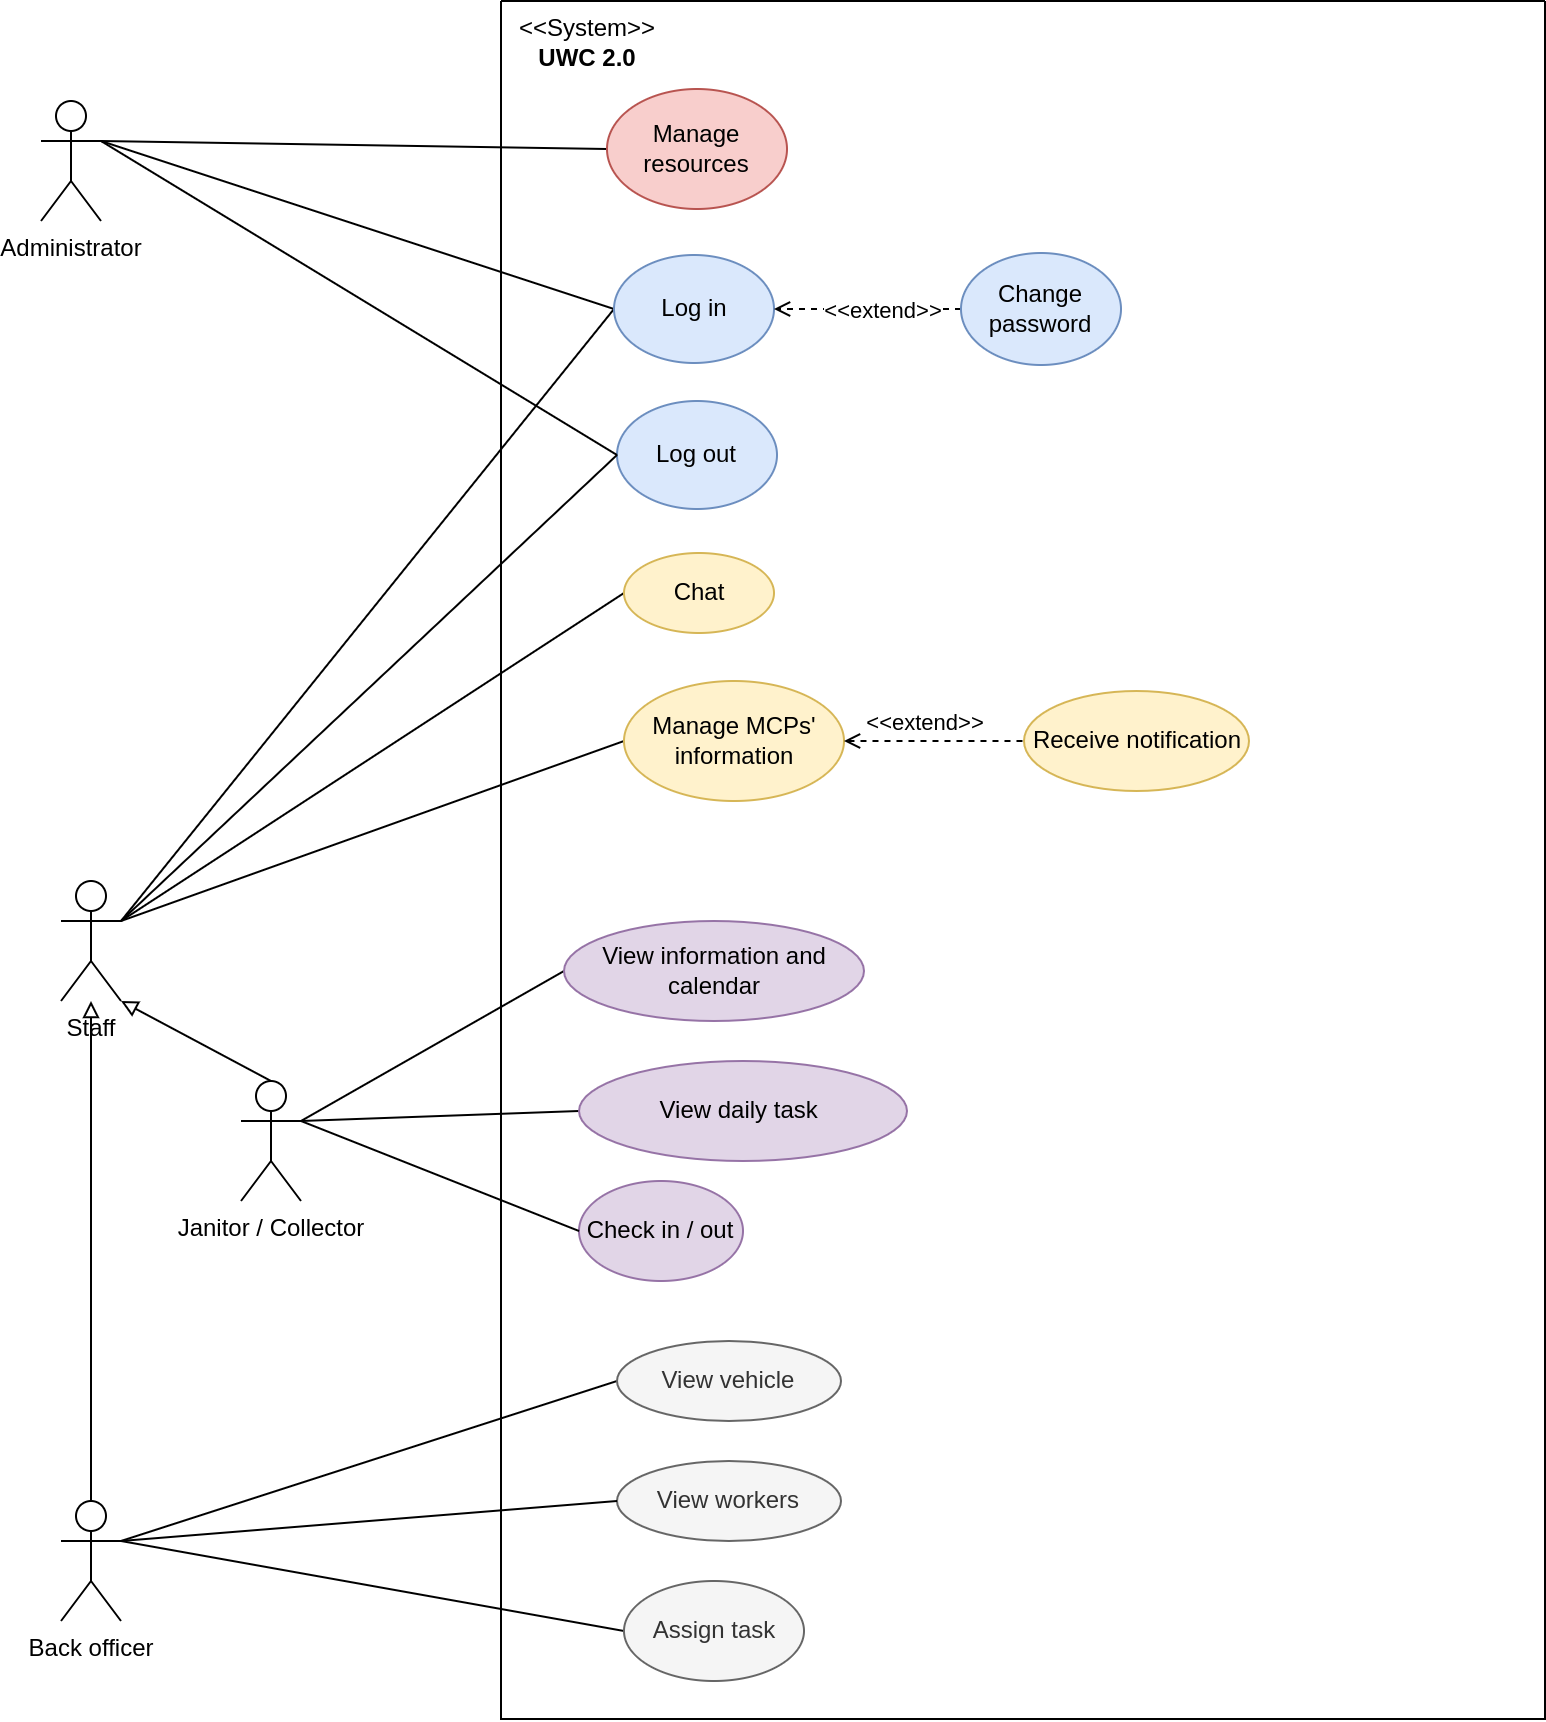
\includegraphics[width=0.93\linewidth]{imgs/use-case diagram/main_uc.png}
        \caption{Use-case diagram tổng quát của hệ thống}
    \end{figure}

    \begin{tblr}{
        width=1\linewidth,
        hlines,
        vlines,
        colspec={X[3]X[7]},
        columns = {valign = m, },
        row{1} = {halign = c, valign = m, bg = lightgray, fg = black},
    }
        {\textbf{Use case name} & \textbf{Manage resources}}  \\
        Description	& Quản lý tài nguyên của công ty \\
        Actor & Người quản lý (Administrator) \\
        Trigger & Người quản lý ấn vào phần quản lý tài nguyên  \\
        Pre-condition & Người quản lý đã đăng nhập và đang ở màn hình chính\\
        Post-condition & Người quản lý được đưa vào trang quản lý tài nguyên\\
        Normal flow &   		1. Hệ thống hiển thị giao diện quản lý tài nguyên \newline
                                2. Quản lý thực hiện việc quản lý tài nguyên \\
        Alternative flow  & 	none \\
        Exception flow & none\\
    \end{tblr}
   
    \vspace{1cm}
   
    \begin{tblr}{
        width=1\linewidth,
        hlines,
        vlines,
        colspec={X[3]X[7]},
        columns = {valign = m, },
        row{1} = {halign = c, valign = m, bg = lightgray, fg = black},
    }
        {\textbf{Use case name} & \textbf{Log in}}  \\
        Description	& Đăng nhập vào hệ thống \\
        Actor & Người quản lý (Administrator), nhân viên giám sát (Back officer), nhân viên lái xe rác (Collector), nhân viên thu gom rác (Janitor) \\
        Trigger & Người dùng mở ứng dụng  \\
        Pre-condition & Thiết bị phải có kết nối Internet\\
        Post-condition & Người dùng đăng nhập thành công\\
        Normal flow &   1. Hệ thống hiển thị giao diện đăng nhập \newline
                    	2. Người dùng ghi thông tin về tên tài khoản và mật khẩu \newline
                    	3. Hệ thống kiểm tra thông tin được ghi \newline
                    	4. Hệ thống thông báo đăng nhập thành công \newline
                    	5. Hệ thống hiển thị giao diện màn hình chính \\
        Alternative flow  & Alternative flow thứ 1: tại bước 2 \newline
                        	1a. Người dùng chọn lưu tài khoản \newline
                        	Tiếp tục bước 3 \newline
                        	1b. Hệ thống lưu lại tài khoản \newline
                        	Tiếp tục bước 4 \\
        Exception flow & 	Exception flow thứ 1: tại bước 3 \newline
                        	1a. Nếu không tìm thấy tài khoản, sai mật khẩu, thông báo cho người dùng \newline
                        	Quay lại bước 2 \\
        Extended points & Change password \\
    \end{tblr}
   
    \vspace{1cm}
    \begin{tblr}{
        width=1\linewidth,
        hlines,
        vlines,
        colspec={X[3]X[7]},
        columns = {valign = m, },
        row{1} = {halign = c, valign = m, bg = lightgray, fg = black},
    }
        {\textbf{Use case name} & \textbf{Change password}}  \\
        Description	& Thay đổi mật khẩu của tài khoản \\
        Actor & Người quản lý (Administrator), nhân viên giám sát (Back officer), nhân viên lái xe rác (Collector), nhân viên thu gom rác (Janitor) \\
        Trigger & Người dùng ấn vào nút quên mật khẩu  \\
        Pre-condition & Người dùng đang ở phần đăng nhập \\
        Post-condition & Mật khẩu được thay đổi thành công \\
        Normal flow &   1. Hệ thống hiển thị thay giao diện thay đổi mật khẩu \newline
                    	2. Người dùng nhập tên tài khoản \newline
                    	3. Hệ thống kiểm tra tài khoản \newline
                    	4. Người dùng nhập mã mật khẩu mới \newline
                    	5. Hệ thống kiểm tra mật khẩu mới \newline
                    	6. Hệ thống thông báo đổi mật khẩu thành công \newline
                    	7. Hệ thống quay lại trang đăng nhập \\
        Alternative flow  & none \\
        Exception flow & 	Exception flow thứ 1: tại bước 3 \newline
                            1a. Nếu tài khoản không tồn tại, thông báo cho người dùng \newline
                            Quay lại bước 2 \newline
                           
                            Exception flow thứ 2: tại bước 5 \newline
                            2a. Nếu mật khẩu không đúng quy đinh, thông báo cho người dùng \newline
                            Quay lại bước 4 \\
    \end{tblr}
   
    \vspace{1cm}
    \begin{tblr}{
        width=1\linewidth,
        hlines,
        vlines,
        colspec={X[3]X[7]},
        columns = {valign = m, },
        row{1} = {halign = c, valign = m, bg = lightgray, fg = black},
    }
        {\textbf{Use case name} & \textbf{Log out}}  \\
        Description	& Đăng xuất khỏi phiên làm việc \\
        Actor & Người quản lý (Administrator), nhân viên giám sát (Back officer), nhân viên lái xe rác (Collector), nhân viên thu gom rác (Janitor) \\
        Trigger & Người dùng ấn vào nút đăng xuất  \\
        Pre-condition & Người dùng đã đăng nhập, và đang ở màn hình chính \\
        Post-condition & Tài khoản được đăng xuất khỏi hệ thống \\
        Normal flow &   1. Người dùng ấn vào menu \newline
                    	2. Người dùng chọn đăng xuất \newline
                    	3. Hệ thống hiện thị form xác nhận đăng xuất \newline
                    	4. Hệ thống xóa phiên làm việc  \newline
                    	5. Hệ thống quay trở lại trang đăng nhập \\
        Alternative flow  & Alternative flow thứ 1: tại bước 3 \newline
                            1a. Nếu người dùng chọn hủy, quay lại màn hình chính \\
        Exception flow & none\\
    \end{tblr}
   
    \begin{tblr}{
        width=1\linewidth,
        hlines,
        vlines,
        colspec={X[3]X[7]},
        columns = {valign = m, },
        row{1} = {halign = c, valign = m, bg = lightgray, fg = black},
    }
        {\textbf{Use case name} & \textbf{Chat}}  \\
        Description	& Nhân viên liên lạc với nhau \\
        Actor & Nhân viên (Staff) \\
        Trigger & 	Nhân viên ấn vào phần liên hệ \\
        Pre-condition & Người dùng đã đăng nhập\\
        Post-condition & Tin nhắn được gửi thành công \newline
                         Nhân viên nhận và đọc được tin nhắn \\
        Normal flow &   1. Hệ thống lấy thông tin về các nhân viên \newline
                    	2. Hệ thống hiển thị danh sách các nhân viên \newline
                    	3. Người dùng chọn nhân viên muốn liên hệ \newline
                    	4. Hệ thống hiển thị giao diện nhắn tin \newline
                    	5. Người dùng nhập tin nhắn \newline
                    	6. Người dùng nhấn gửi \newline
                    	7. Hệ thống ghi nhận tin nhắn và gửi cho người được nhắn \\
        Alternative flow  & none \\
        Exception flow & none \\
    \end{tblr}
   
    \vspace{1cm}
    \begin{tblr}{
        width=1\linewidth,
        hlines,
        vlines,
        colspec={X[3]X[7]},
        columns = {valign = m, },
        row{1} = {halign = c, valign = m, bg = lightgray, fg = black},
    }
        {\textbf{Use case name} & \textbf{Manage MCP's information}}  \\
        Description	& Xem thông tin về các MCPs \\
        Actor & Nhân viên (Staff) \\
        Trigger & 	Nhân viên ấn vào mục tổng quan MCPs \\
        Pre-condition & Nhân viên đã đăng nhập và đang ở màn hình chính \\
        Post-condition & Thông tin về MCP được hiển thị thành công \\
        Normal flow &   1. Hệ thống lấy thông tin các MCPs \newline
                    	2. Hệ thống hiện thị danh sách các MCPs \newline
                    	3. Nhân viên chọn 1 MCP bất kì \newline
                    	4. Hệ thống hiển thị thông tin chi tiết của MCPs vừa được chọn \\
        Alternative flow  & none \\
        Exception flow & none \\
        Extended points & Receive notification \\
    \end{tblr}
   
    \begin{tblr}{
        width=1\linewidth,
        hlines,
        vlines,
        colspec={X[3]X[7]},
        columns = {valign = m, },
        row{1} = {halign = c, valign = m, bg = lightgray, fg = black},
    }
        {\textbf{Use case name} & \textbf{Receive notification}}  \\
        Description	& Cập nhật tình trạng của MCP \\
        Actor & Nhân viên (Staff) \\
        Trigger & none \\
        Pre-condition & Nhân viên đã đăng nhập \\
        Post-condition & Thông báo được nhận bởi nhân viên \\
        Normal flow &   1. Hệ thống truy cập vào dữ liệu về MCPs \newline
                    	2. Hệ thống lấy thông tin về dung tích của MCPs \newline
                    	3. Hệ thống gửi thông báo về cho người dùng \newline
                    	4. Người dùng nhận được thông báo \\
        Alternative flow  & none \\
        Exception flow & none \\
    \end{tblr}
   
    \vspace{1cm}
    \begin{tblr}{
        width=1\linewidth,
        hlines,
        vlines,
        colspec={X[3]X[7]},
        columns = {valign = m, },
        row{1} = {halign = c, valign = m, bg = lightgray, fg = black},
    }
        {\textbf{Use case name} & \textbf{View information and calendar}}  \\
        Description	& Công nhân xem thông tin và lịch làm trong tuần \\
        Actor & 	Nhân viên lái xe rác (Collector), Nhân viên thu gom rác (Janitor) \\
        Trigger & 	Công nhân ấn vào phần thông tin và lịch làm \\
        Pre-condition & Công nhân đã đăng nhập và đang ở màn hình chính \\
        Post-condition & Công nhân xem được thông tin và lịch làm của mình \\
        Normal flow &   1. Hệ thống lấy thông tin và lịch làm \newline
                    	2. Hệ thống hiển thị giao diện bao gồm 2 tab (thông tin chung, lịch làm) 	mặc định ở thông tin chung \newline
                    	3. Công nhân xem thông tin của bản thân\\
        Alternative flow  & Alternative flow thứ 1: Tại bước 2 \newline
                    	    1a. Người dùng chọn tab lịch làm \newline
                    	    1b. Hệ thống hiển thị giao diện về lịch làm việc trong tuần \\
        Exception flow & none \\
    \end{tblr}
   
    \begin{tblr}{
        width=1\linewidth,
        hlines,
        vlines,
        colspec={X[3]X[7]},
        columns = {valign = m, },
        row{1} = {halign = c, valign = m, bg = lightgray, fg = black},
    }
        {\textbf{Use case name} & \textbf{View daily task}}  \\
        Description	& Công nhân xem chi tiết công việc trong ngày \\
        Actor & 	Nhân viên lái xe rác (Collector), Nhân viên thu gom rác (Janitor) \\
        Trigger & 	Công nhân ấn vào phần nhiệm vụ hôm nay\\
        Pre-condition & Công nhân đã đăng nhập và đang ở màn hình chính \\
        Post-condition & Nhiệm vụ cụ thể trong ngày được hiện lên màn hình \\
        Normal flow &   1. Hệ thống lấy thông tin làm việc trong ngày \newline
                    	2. Hệ thống hiển thị thông tin làm việc \newline
                    	3. Người dùng đọc được thông tin làm việc\\
        Alternative flow  & none \\
        Exception flow & none \\
    \end{tblr}
   
    \vspace{1cm}
    \begin{tblr}{
        width=1\linewidth,
        hlines,
        vlines,
        colspec={X[3]X[7]},
        columns = {valign = m, },
        row{1} = {halign = c, valign = m, bg = lightgray, fg = black},
    }
        {\textbf{Use case name} & \textbf{Check in/out}}  \\
        Description	& Nhận và đánh dấu hoàn thành công việc \\
        Actor & 	Nhân viên lái xe rác (Collector), Nhân viên thu gom rác (Janitor) \\
        Trigger & 		Công nhân chọn nhận công việc \\
        Pre-condition & Công nhân đang ở phần thông tin nhiệm vụ chi tiết \\
        Post-condition & Nhiệm vụ được nhận / được hoàn thành \\
        Normal flow &   1. Công nhân xác nhận nhiệm vụ \newline
                        2. Hệ thống ghi nhận công nhân đã xác nhận \\
        Alternative flow  & Alternative flow thứ 1: tại bước 1 \newline
                        	1a. Công nhân ấn hoàn thành nhiệm vụ \newline
                        	1b. Hệ thống ghi nhận \\
        Exception flow & none \\
    \end{tblr}
   
    \begin{tblr}{
        width=1\linewidth,
        hlines,
        vlines,
        colspec={X[3]X[7]},
        columns = {valign = m, },
        row{1} = {halign = c, valign = m, bg = lightgray, fg = black},
    }
        {\textbf{Use case name} & \textbf{View workers}}  \\
        Description	& Xem thông tin công nhân và lịch làm của họ \\
        Actor & 	Nhân viên giám sát (Back officer) \\
        Trigger & 	Nhân viên giám sát ấn vào mục quản lý nhân viên \\
        Pre-condition & Nhân viên giám sát đã đăng nhập và đang ở màn hình chính \\
        Post-condition & Thông tin chi tiết và lịch làm việc trong tuần của công nhân được hiển thị \\
        Normal flow &   1. Hệ thống lấy dữ liệu của nhân viên \newline
                    	2. Hệ thống hiển thị danh sách tên các nhân viên \newline
                    	3. Nhân viên giám sát chọn một nhân viên \newline
                    	4. Hệ thống hiển thị thông tin chi tiết của nhân viên \\
        Alternative flow  & Alternative flow thứ 1: tại bước 4 \newline
                        	1a. Người dùng chọn qua mục lịch làm việc \newline
                        	1b. Hệ thống lấy thông tin về lịch làm việc của nhân viên \newline
                        	1c. Hệ thống hiển thị lên màn hình \\
        Exception flow & none \\
    \end{tblr}
   
    \vspace{1cm}
    \begin{tblr}{
        width=1\linewidth,
        hlines,
        vlines,
        colspec={X[3]X[7]},
        columns = {valign = m, },
        row{1} = {halign = c, valign = m, bg = lightgray, fg = black},
    }
        {\textbf{Use case name} & \textbf{View vehicle}}  \\
        Description	& Xem thông tin của các phương tiện \\
        Actor & 	Nhân viên giám sát (Back officer) \\
        Trigger & 	Nhân viên giám sát ấn vào mục theo dõi phương tiện\\
        Pre-condition & Nhân viên giám sát đã đăng nhập và đang ở màn hình chính \\
        Post-condition & Thông tin phương tiện được hiển thị trên màn hình \\
        Normal flow &   1. Hệ thống truy cập vào dữ liệu về phương tiện \newline
                    	2. Hệ thống hiển thị các phương tiện \newline
                    	3. Người dùng chọn một phương tiện bất kì \newline
                    	4. Hệ thống hiện thị thông tin chi tiết của phương tiện \\
        Alternative flow  & none \\
        Exception flow & none \\
    \end{tblr}
    \newpage   
